\documentclass[a4paper,11pt]{report}

\usepackage[utf8]{inputenc}
\usepackage[T1]{fontenc}
\usepackage[francais]{babel}
\usepackage{amsfonts}
\usepackage{amsmath}
\usepackage{amsthm}
\usepackage[pdftex]{graphicx}
\usepackage{float}
\usepackage{listings}
\usepackage{fullpage}
%
\newcommand{\alinea}{
\hspace*{0.5cm}}
%
\renewcommand{\thesection}{\arabic{section}}
%
\newtheorem{definition}{Definition}
\newtheorem{law}{S.E. law}
%
\title{Basic Principles of Software Evolution: Summary}
\author{Anthony Rouneau}
%
\begin{document}
\maketitle
\newpage
%
\section{Aspects of Software Evolution}
	\subsection{Technical aspects}
		Here are some technical aspects of the
			Software Evolution.
		%
		\begin{itemize}
			\item Version management
			\item Software quality measurement
				and improvement
			\item Legacy systems and migration
			\item Reverse Engineering and program
				comprehension
			\item Model-driven evolution
			\item Change propagation and program
				comprehension
			\item Traceability
			\item Co-evolution
			\item Consistency maintenance
			\item Regression testing
			\item Design for change
			\item Visualisation and statistical
				analysis of evolution histories
			\item Software product lines and 
				product families
		\end{itemize}
		%
		\begin{definition}
			\textbf{Reverse engineering} --
				Process of analysing a project to fully
				understand it and to extract the key
				issues.
		\end{definition}
		%
		\begin{definition}
			\textbf{Re-engineering} -- 
				Horseshoe process (cf. figure
				\ref{fig:reengineering}) that targets
				to rethink a project in order to
				address one or multiple problems.
		\end{definition}
		%
		\begin{figure}[H]
			\centering
			\includegraphics[scale=0.2]{figures/%
			reengineering}
			\caption{Re-engineering}%
			\label{fig:reengineering}
		\end{figure}\noindent
		%
	%
	\subsection{Managerial aspects}
		\begin{itemize}
			\item Evolutionary process model
				\begin{itemize}	
					\item Staged life-cycle
					\item Iterative and incremental 
						process
					\item Agile methods
				\end{itemize}
			\item Software configuration management
				\begin{itemize}
					\item Change management
					\item Version management
				\end{itemize}
			\item Estimation techniques
				\begin{itemize}	
					\item Change impact analysis
					\item Effort estimation
					\item Cost estimation
					\item Change metrics
				\end{itemize}
		\end{itemize}
	%
%
\newpage
%
\section{Software Maintenance}\noindent
	The software maintenance is used
		to avoid \textbf{large} software to become 
		legacy systems. In fact, adding
		new functionalities without 
		considering code quality gives rise
		to \textbf{technical debt}.
	\begin{definition}
		\textbf{Technical debt} -- 
			Lack of quality in the code due to 
			modifications done in a hurry.
			The project is unclean while the debt
			has not been paid back through 
			re-engineering.
	\end{definition}
	%
	\begin{definition}
		\textbf{Software maintenance (1)} -- 
			The process of modifying a software 
			system or component after delivery 
			to correct faults, improve 
			performance or other attributes, 
			or adapt to a changed environment
	\end{definition}
	%
	\begin{definition}
		\textbf{Software maintenance (2)} -- 
			The software product undergoes 
			modification to code and associated 
			documentation due to a problem or
			the need for improvement. 
			The objective is to modify
			the existing software product 
			while preserving its integrity
	\end{definition}\noindent
	%
	The software change is :
	\begin{itemize}
		\setlength{\itemsep}{0pt}		
		\setlength{\parskip}{0pt}		
		\setlength{\parsep}{0pt}	
		\item \textbf{Unpredictable} --
			All the changes and bugs can not be
			anticipated in the design.
		\item \textbf{Expensive} --
			You generally don't get paid to solve bugs but
			to develop as fast as possible.
		\item \textbf{Difficult}-- The errors are hard
			to find and the source code can be messy.
	\end{itemize}
	%
	\subsection{Legacy system}
		Characteristics : 
		\begin{itemize}	
			\item Original developers no longer
				available
			\item Outdated development methods
				used
			\item Extensive patches and modifications 
				have been made
			\item Missing or outdated documentation
		\end{itemize}
	%
	\subsection{Parnas' ageing software}
		Symptoms :
		\begin{itemize}
			\item Lack of knowledge
				\begin{itemize}
					\item Insufficient, inconsistent or
						obsolete documentation
					\item Departure of original 
						developers
					\item Disappearance of inside 
						knowledge about the system
					\item Missing tests
				\end{itemize}
			\item Code symptoms
				\begin{itemize}
					\item Duplicated code, code smells, 
						lack of modularity
					\item Lack of overall structure 
						or architecture
				\end{itemize}
			\item Process symptoms
				\begin{itemize}	
					\item Constant need for bug fixes
						Too long time to fix bugs or to 
						add new functionality
					\item Difficult to separate
						functionalities
				\end{itemize}
		\end{itemize}
		%
	%
	\newpage
	%
	\subsection{Necessity of software change}
		Software change is inevitable because:
		%
		\begin{itemize}
			\item New requirements emerge when the 
				software is used or developed.
			\item The business environment changes.
				\begin{itemize}	
					\item New customers
					\item New demands
					\item Organisational changes
					\item Competitors
				\end{itemize}
			\item Errors must be repaired
				\begin{itemize}
					\item Bug fix routine
					\item Emergency fix
				\end{itemize}
			\item Hardware changed
			\item Improvements needed in efficiency
			\item New technologies have to be used
			\item Changes in data formats
				\begin{itemize}
					\item New standards
					\item New currency, ...
				\end{itemize}
		\end{itemize}
		%
	%
	\subsection{Types of software maintenance}
		\begin{itemize}
			\item \textbf{Adaptive} -- 
				Adapt a software after delivery 
				to support new technologies
			\item \textbf{Corrective} -- 
				Repair errors discovered after delivery
			\item \textbf{Perfective} -- 
				Add new functionalities to the 
				software or improve it after delivery\\
				\alinea\alinea\alinea
				\alinea
				\alinea$\Longrightarrow$ \textit{main reason}
			\item \textbf{Preventive} --
				Correct latent faults before they
				become effective ones.
		\end{itemize}
		%
		\begin{center}
			\begin{tabular}{|c|c|c|}
				\hline
				\textit{When? / Why?} & 
					\textbf{Correction} &
					\textbf{Enhancement}\\
				\hline
				\textbf{Proactive} (before it happens) & 
					Preventive & Perfective\\
				\hline		
				\textbf{Reactive} (after it happened) & 
					Corrective & Adaptive\\			
				\hline
			\end{tabular}
		\end{center}
		%
		\begin{figure}[H]
			\centering
			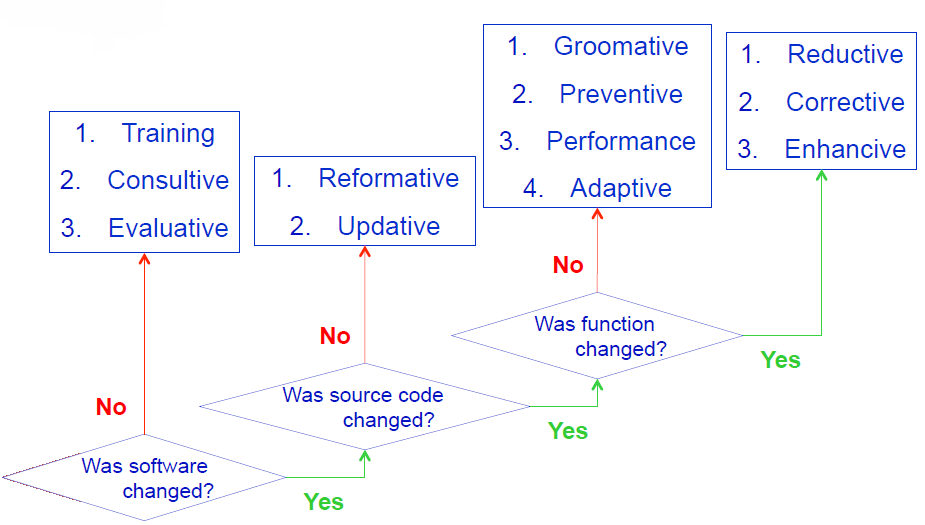
\includegraphics[scale=0.6]{figures/types.PNG}
		\end{figure}\noindent
		%
	%
%
\end{document}
